\chapter{使用した技術}
%rosについてもっと深堀する
%例:パッケージの作り方,ノードの作り方,Publisherとはなにか,サブスクライバーとはなにか
%ROSのPublisherとサブスクライバーの作り方,mROS 2の作り方embeddedRTPSについても話せるとよい
%C++とpythonの違いを述べる.本実装ではなぜC++を選択したのかを書く
%ついでにServiceとActionについても述べる
%messageの中身についても語りたい.後で説明が楽になる
\label{sec:usage}
\section{ROS 2}
ロボットシステムを開発するにあたって現在はROS 2が主流であるが,その前身であるROSは,スタンフォード人工知能研究所の研究プロジェクトとから移管されたWillow Garage社によって開発が始まったロボットソフトウェア開発基盤である.
最初の正式なディストリビューション版は,2010年3月にリリースされたBox Turtleで,その後,Fuerte,Groovy,Hydro,Indigo,Jade,Kinetic,Lunar,Melodic,Noetic,Foxy,Galactic,Humbleといったバージョンがリリースされている.
ROSの利点は,分散型ロボットシステムの実現に向いている通信ミドルウェアの実装やRTPS(Real Time Publish Subscribe)通信プロトコル,プロジェクト管理やデバックおよびシミュレーションなどのための広範囲なツール群,豊富なOSS(Open Source Software)のパッケージやライブラリ,世界規模の活発なオープンソース開発コミュニティという4つの側面にある[8].\\
 パッケージやライブラリに関しては公式のものだけでも多種多様であり,ロボット本体の制御,モーターの制御,センサーの制御,画像処理,音声認識,自律走行,SLAM(Simultaneous Localization and Mapping)など,ロボットシステムに必要な機能を網羅している.
短期間で機能の大枠を組み立てることができるため,研究開発,教育,産業用途においても,幅広い分野で利用されている.\\
 ROSすでに10年以上の歴史を持っており,ロボット工学の発展に大きく貢献してきた.
日本の企業ではソニーのaiboの事例がROSを使った製品として代表的であり,他の企業でも商用商品に採用されることも多い.
ロボット開発を取り巻く環境やROSが研究用から商用にも活用され始めるという変遷を受け,2014年より第2世代バージョンであるROS 2の開発が始まった.
これはROS 1は研究用途においては十分な性能を持っていたが,商用製品においてはリアルタイム性やセキュリティの問題があった.
ROS 1の設計は以下のようにされている.
    \begin{itemize}
        \item 単一のロボットで動作することを想定
        \item 多くのリソースを抱えているマシン上で動作されることを想定
        \item リアルタイム性は考慮しない
        \item 優れたネットワーク上で動作されることを想定(有線接続など)
        \item 研究,主に学術的なアプリケーションを想定
        \item 規制や禁止事項がなく,最大限の柔軟性がある(プログラムがmain()から始まることを決定していないなど)
    \end{itemize}
そのため,産業用に利用されることが増えるとこの設計が問題になることが多かった.
\\ ROS 1が抱える課題として以下のようなものがある.
   \begin{enumerate}
       \item メッセージ通信の仲介役としてROS Masterが必要である.ROS Masterが何らかの原因でダウンすると,全てのプロセスがダウンしてしまうという問題がある.
       \item リアルタイム性を考慮していない設計になっている.
       \item メッセージを暗号化せずに送受信を行っているため,セキュリティに問題がある.
       \item 実行するマシンにリソースが少ないと動作が不安定になるという問題がある.
       \item Ubuntu(Linux)でないと使いにくい
   \end{enumerate}
ROS 2では,ROS 1の上記の問題を解決するため,リアルタイムおよび組込みシステム向けのDDS(Data Distribution Service)[7]と呼ばれる通信ミドルウェアを採用し,通信の信頼性を確保するためのQoS(Quality of Service)制御の機能を導入した.\\
 このDDSの採用により,(1)の問題点がなくなり,QoSとDDSの組み合わせにより,(2)に対してリアルタイム性の実現を目指した.(3)のセキュリティの問題はROS 2でメッセージの暗号化が施されたことにより解決した.また,(4)に対応するためにリソースの少ないマシンで動作できるように開発されている.さらにUbuntu以外のOSにも対応した.
\\ ROS 2の構成を図1に示す.
ROS 2では図のようにユーザーが実装するアプリケーション層があり,その下にクライアントライブラリであるrclの層がある.rclクライアントライブラリ層には通信概念を公開するAPIの定義がされており,DDSの上に構築された.rclは,C++,Pythonといった各プログラミング言語用のクライアントライブラリに共通する機能を提供しているAPIである.その下部にDDSとrmw(ROS Middleware Interface)がある.DDSはリアルタイム通信を行うためのAPIとプロトコルを提供している国際ミドルウェア標準[].rmwは様々な種類のDDS実装,各backendの差を吸収,最適化を施している層であり,rclクライアントライブラリに対して共通のインタフェースを提供している.RTPSはDDSから呼び出されるtranceport層に位置する通信プロトコルである.backendとして,RTOSやPOSIX,NoCなどのROS 2は様々な環境で動作するためを表す層がある.
\\ このように,従来のROS 1では難しかったロボットシステムでもROS 2を使うことで,個々のロボットが独立して動作するだけでなく,複数のロボットが協調して動作する分散型ロボットシステムの開発が可能になった.
\\ 2015年8月には最初のディストリビューションであるアルファ版がリリースされ,2017年の12月にROS 2が本リリースされた.
2023年のMetrics Report[]によると,ROSは550,365,601回ダウンロードされている.
そのうち30\%がROSのディストリビューションであるNoeticで,32\%がROS 2のディストリビューションであるhumbleである.
2023年でROSはNoetic,ROS 2はhumbleが主流のディストリビューションであった.
本研究はubuntu 22.04でリリースされたROS 2のhumbleディストリビューションを使用している.
\subsection{PublisherとSubscriber}
ROSでは基本的なノード間のデータ通信としてPublish/Subscribe(Pub/Sub)通信型の非同期な通信プロトコルを採用している.
データの送信側をPublisher(出版者)とよび,受信側をSubscriber(購読者)と呼ぶ.
通信経路として,トピック(Topic)を介した通信が行われる.
トピックで送受信されるデータはメッセージ(Message)と呼ばれ,車輪の角速度や回転量,現在位置の3次元座標など,基本型を組合せた任意の型を定義することができる.
同じ名前のトピックに対して,様々な個数や種類のノードが任意のタイミングで登録,変更,削除ができる.
さらに,メッセージの型が一致していれば,通信が行われる.
Publisher側は自由なタイミングでTopicに向けて通信を行い,非同期に動作するSubscriber側は,Publisherからメッセージを受け取った際に対応するコールバック関数が実行される.
ノードはPublisherやSubscriber,またその両方をプログラム次第で変化できるため,ユーザが考えたオリジナルのノードを作成することができる.
この仕様のため,ノード同士の依存が少なくなり,ロボットシステム全体の機能の追加や削除が容易である特性は,柔軟なロボットシステムの構築の一助となる.
ROS 2でPublisherを作成する際,C++でrclcpp::Nodeクラスの継承からcreate\_publisher(),Pythonでimport rclpy後に.create\_publisher()を行うことでPublisherを作成することができる.
同様にSubscriberはC++でrclcpp::Subscriptionクラスを使用してcreate\_subscriber(),Pythonでimport rclpy後にcreate\_subscriberを記述することでSubscriberを作成できる.
\subsection{ServiceとAction}
ROS 2では,Publisherとサブスクライバー以外にもService通信とAction通信がある.
Service通信は,サーバーとクライアントの2つのノード間でリクエストとレスポンスをやり取りする通信である.
これは既存のクライアント・サーバーモデル[15]によく似ており,Subscribeするのではなく,ノードがメッセージの値を欲しいタイミングでリクエストする仕組みになっている.
そのため,ロボットに対する命令やデータの取得,計算結果を受け渡しに適しており,Service通信はリアルタイム性や連続的なデータには向かないが,確実に応答するというロボットシステムにおいて重要な役割を果たす.
さらに,Service通信は同期的な通信であるため,Service通信を行うノードは,Service通信が完了するまで他の処理を行うことができない.
そのため,クライアントの処理を間接的にブロックすることができる.
一方,Action通信は,Service通信と同様にサーバーとクライアントの2つのノード間でリクエストとレスポンスをやり取りする通信である.
しかし,Action通信はService通信と異なり,リクエストに対するレスポンスを即座に返すのではなく,リクエストに対するレスポンスを返すまでの間に,進捗状況を返すことができる.
この通信方式によって,長時間のタスクやフィードバックが可能なタスク,中断可能なタスクに適しているため,開発者は柔軟性を保ちながら,ロボットシステムを構築することができる.
さらに,Action通信は非同期的な通信であるため,Action通信を行うノードは,Action通信が完了するまで他の処理を行うことができる.
これによって,複雑なタスクを行うノードでもAction通信を用いることで同時に処理することが可能であり,多くのリソースがあるマシンで高度なノードを動作させることができる.
% \subsection{オーバーレイとアンダーレイ}
% また,ROS 2には重要な概念にアンダーレイとオーバーレイがある.
% アンダーレイは,完成されたパッケージをインストールするワークスペースであり,安定した環境をオーバーレイに提供するためにある.
% オーバーレイは,ユーザー自身で作成したパッケージを扱うワークスペースであり,先ほどのros2\_wsはオーバーレイにあたる.
% ROS 2ではユーザーが作るノードやパッケージをオーバーレイに作成し,必要に応じてアンダーレイのパッケージを参照して使用するのが一般的である.
% このオーバーレイ上でユーザはcolcon buildを実行し,パッケージをビルドする.
% ユーザーはパッケージをビルドした後,すぐに実行することができない.ROS 2ではsourceコマンドを用いてオーバーレイ環境を読み込むことでアンダーレイがオーバーレイより優先されることなく,開発することができる.
% ROS 2においてオーバーレイとアンダーレイは,複雑化するロボットシステムに柔軟性と拡張性をもたらす概念であることがわかる.
% ROS 2のデバック方法として様々なコマンドが用意されており,ros2 topic listというコマンドを実行することで,現在実行されているトピックの一覧を表示することができる.
% ros2 topic echoは,指定したトピックのメッセージを表示することができる.
% また,現在実行されているノードを視覚的に確認できるようにrqt\_graphと呼ばれるものが用意されている.開発者はrqt\_graphを用いて,目に見えないROS 2のノード間の通信を確認することができる.
% こうしたアンダーレイ機能の充実によって,ROS 2はROS 1よりも柔軟性と拡張性を持つことができた.
% \subsection{ROS 2が対応しているDDS}
% ROS 2の通信ミドルウェアであるDDSと通信プロトコルであるRTPSは,通信相手の探索および通信経路の確立を自律的に行う.
% この機能の実現は,RTPSのSPDP(Simple Participant Discover Protocol)とSEDP(Simple Endpoint Discover Protocol)[9]というプロトコルによって行われる.ここで,RTPSでは,ROS 2のノードに相当するものをParticipant(参加者)と呼ぶ.
% 通信相手を探索するためには自身の情報を送信するモジュールをWriter,ほかのParticipantから情報を受け取るモジュールをReaderと呼ぶ.
% SPDPは,Participantの情報を送受信するためのプロトコルであり,SEDPは,Topicの情報を送受信するためのプロトコルである.
% この通信のエンドポイントは,Participant同士のPublish,Subscribeである.
% \\ RTPSをOSI参照モデルに例えるとtransport層に位置し,UDP/IPの上に実装されている.UDP通信にはパケットの到着に関する保証がないが,ROS 2のDDSではこれを補助するQoS(Quality of Service)制御の機能がある.
% QoS制御は,サブスクライバ,パブリッシャごとに設定でき,厳格な条件であればRELIABLE(信頼性の高い通信)を,緩やかな条件であればBEST EFFORT(ベストエフォート通信)を選択することができる.
% ROS 2のデフォルトDDSであるFastRTPS[10]では,QoS制御の機能が実装されており,各ノードが通信するときのQoS設定はRELIABLEである.
% ROS 2にはデフォルトでFastRTPSというDDSが実装されている.
% DDSとは,OMG(Object Management Group)が定めたデータ交換のための仕様である.これによって分散型ネットワークでも効率的に通信が可能になっている.
% FastRTPSのほかにも,RTI Connext DDS[11]やeProsima Micro XRCE-DDS[12]というDDSがROS 2に対応している.
% Ubuntu22.04のROS 2 humbleでは,FastRTPSはもちろんのこと,デフォルトでEcripse Cyclone DDS[13],Gurum DDS[14],RTI Connext DDSがインストールできる.%リファレンス1[https://docs.ros.org/en/humble/Installation/DDS-Implementations.html#ubuntu-linux-source-install].


\section{mROS 2}
\begin{figure}[ht]
    \centering
    \begin{minipage}{.48\textwidth}
        \centering
        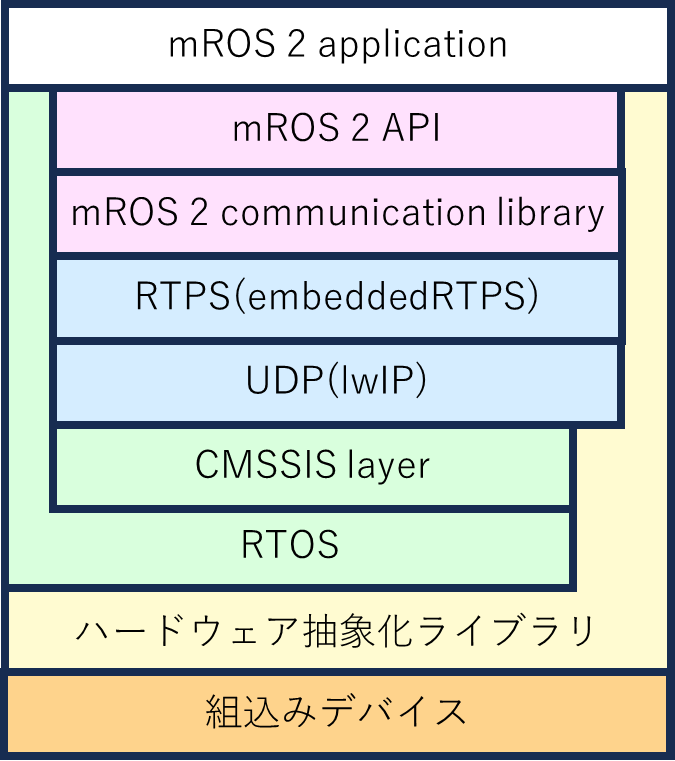
\includegraphics[width=0.9\linewidth]{images/fig1_mros2_b.png}
        \caption{mROS 2の内部構成}
        \label{fig:subfig_a}
    \end{minipage}
    \hfill
    \begin{minipage}{.48\textwidth}
        \centering
        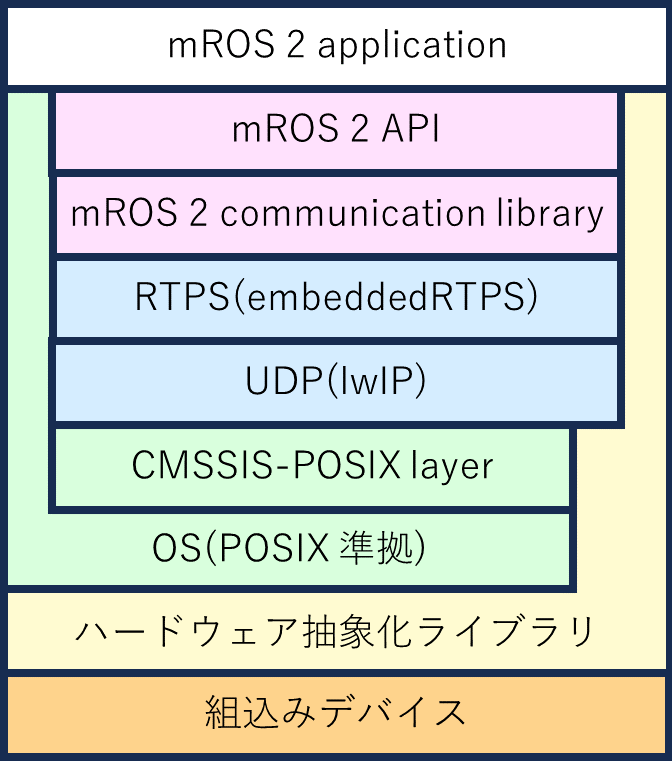
\includegraphics[width=0.9\linewidth]{images/fig1_mros2posix_a.png}
        \caption{mROS 2-POSIXの内部構成}
        \label{fig:subfig_b}
    \end{minipage}
\end{figure}
mROS 2は,ROS 2ノードの軽量実行環境である.
ROS 2を採用するロボットシステムにおいて通信方式とメモリ軽量な実行環境を確立することができる組み込み技術を導入することにより,分散型のロボットシステムにおける応答性やリアルタイム性の向上,消費電力の削減が可能になる.
mROS 2は汎用OS上で実行されるROS 2ノードと通信できることを目的として実装された.
そのため,Pub/Sub通信の相手と経路を自律的に探索できるように設計され,ROS 2およびRTPSの利点が,組み込み技術導入時に損なわれないようになっている.
ROS 2に対応しているDDSの種類として,FastRTPS,RTI Connext DDS,eProsima Micro XRCE-DDSを挙げたが,既存の組込みデバイス向けのROS 2ノード実行環境であるmicro-ROS[16]がある.
micro-ROSはRTPSの軽量規格であるDDS-XRCE(DDS For Extremely Resource Constrained Enviroments)の実装であるMicro XRCE-DDSを採用している.
Micro XRCE-DDSは,ホストとしてROS 2ノードを実行するデバイスと通信する際に,Agentノードと呼ばれるノードの稼働が必要となる.
通信の仲介の役割をAgentノードは担っており,Agentノードは,ホストデバイス上のROS 2ノードとRTPSに則った通信,組み込みデバイス上のノードとXRCEに則った通信をそれぞれ行うため,
応答性とリアルタイム性の低下が懸念される.また,複数の組み込みデバイスを用いる場合,Agent ノードは分散型システム全体の通信を仲介するため,Agentノードの数が増えると通信の遅延が増加する.
そのためmROS 2は,DDSとしてXRCE-DDSを採用せず,embeddeRTPS[17]を採用している.
embeddeRTPSは,一つのDomainクラスからParticipant,Writer,Readerの3つのインスタンスが生成される.つまり,初期化処理の段階でembeddedRTPSの提供するPub/Sub通信が利用できるようになる.
これによってXRCE-DDSのようにAgentノードが必要なく,組み込みデバイス上での通信の遅延を抑えることができる.
このembeddeRTPSが採用されたのは通信の遅延を抑えることができるだけではない.
このRTPSは,SPDPとSEDPが実装されており,通信の宛先や受け手として自立性を確保できるRTPSであること点である.
また,ROS 2で代表的なFastRTPSと通信の確認ができているため親和性が高い点も上げられる.
以上の設計思想によりmROS 2は,計算資源の限定的な組み込みデバイス上での稼働を想定した組込みデバイスのリアルタイム性の向上および消費電力の削減ができるソフトウェア基盤である.
\subsection{mros2の内部構成}
図2.1にmros2の内部構成を示す.
ユーザーアプリケーションからの階層順で,mROS 2通信ライブラリ,通信プロトコルスタック,RTOS,ハードウェア抽象化ライブラリによって構成される.
mROS 2通信ライブラリは,ユーザアプリケーションに対して,ROS 2通信のトピックに関する基本的なAPIを提供している.
主なAPIとして void mros2::init(),void mros2::Node::create\_node(),void mros2::Publisher::create\_publisher(),void mros2::Subscriber::create\_subscriber()がある.
通信プロトコルスタックには,C++で実装されたembeddedRTPSを採用している.先ほど述べたようにこのRTPSにはSPDPとSEDPが実装されており,計算資源の限定的な組込みデバイス上での稼働を想定した設計であるかつ,ROS 2の代表的なRTPSであるFastRTPSと通信の確認できているという理由がある.
UDPについては組込み向けのCによる軽量実装であるlwIP[18]が採用されている.
RTOSには,TOPPERS/ASP3カーネル[19]が採用されており,高分解能タイマやティックレスの低消費電力な処理遅延機能など,高いリアルタイム性と安全性が求められる軽量な組込みシステムに適した設計がなされている.
lwipはCMSIS-RTOS APIに依存しているため,それぞれのAPI差分を吸収するラッパが用意されている.
\subsection{mROS 2の通信機能}
mROS 2の通信機能は,mROS 2の通信ライブラリにあるinit task(初期化処理)とRTPS/UDPと通信ライブラリを介するwrite task(Publish処理)とreader task(Subscribe処理)の3つのタスクに分けられる.
またアプリケーション層にあるuser task(ユーザーアプリケーション)という開発者が実装するタスクがある.
user taskは,ROS 2のノードに相当している.Pub/Sub通信を行うアプリケーションである.
mROS 2のAPIを介してPublishやSubscribeを行うことができる.
init taskはROS 2としてのノードの情報の初期化を行う.APImros2::init()が呼ばれたときに,対象の組込みデバイスをRTPSのParticipantとして登録する.
writer taskとreader taskに関しては,PublishおよびSubscribeに関する処理を担う.これらのタスクはuser taskからの依頼をmROS 2APIを介して受け,RTPSの該当機能を立ち上げる.
writer taskはPublishの依頼を受けて起動し,reader taskはSubscribeの依頼を受けて起動する.
\subsection{mROS 2-POSIXの内部構成}
mROS 2がPOSIX[20]に対応したのがmROS 2-POSIXである.
\\ 図2.2は,mROS 2-POSIXのソフトウェア構成を示す.mROS 2-POSIXアプリケーション層は,ユーザが実装するROS 2ノードに相当する.
つまり,ROS 2におけるオーバーレイに相当する層である.
mROS 2-POSIX API層および通信ライブラリ層は,メッセージを非同期にPublishやSubscribeするためのコミュニケーションチャネルであるROS 2のTopicに相当するAPIおよび通信機能を提供する階層である.
本階層は,ROS 2のネイティブなクライアント通信ライブラリであるrclcppと互換性を保つように設計されている.
mROS 2通信ライブラリでは,rclcppのうちpub/sub通信の基本的な機能のみ実装されている.
利用可能な機能は制限されているものの,組込み技術を導入するROS 2開発者は,汎用OS向けのプログラミングスタイルを踏襲しながらC++によってmROS 2のアプリケーションを実装できる.
そのためmROS 2-POSIXはService通信やAction通信には対応していない.
\\ RTPSプロトコルスタックにはUDPでパブリッシャとサブスクライバC++実装のembeddedRTPSが採用されている.
UDPについては組込み向けのC実装であるlwIPが採用されている.
通信層のembeddedRTPSおよびlwIPはCMSAIS-POSIX[21]に依存しており,図1(b)に示すmROS 2のCMSIS-RTOSを互換した層になっている.
最下層にはハードウェアを抽象化したライブラリがある.
\\ mROS 2-POSIXは図2に示す実行方式を採用している.
リアルタイムOSでは,組込みマイコンを実行資源の管理対象として,タスク単位でアプリケーションが実行される.
POSIXにおいてはタスクに相当する概念はプロセスであり,そこから生成されるスレッドを実行単位として処理が進行している.
しかし,mROS 2-POSIXは実行単位であるノードにPOSIXのスレッドを対応づけ,組込みマイコンでの通信処理におけるイベント割込みについては,POSIX準拠OSにおけるブロッキングAPIの発行に相当させて処理している.
これらの方式によって,mROS 2-POSIXはPOSIX準拠OS上で仮想ROS 2ノードとして軽量環境下で実行することができる.
% \subsection{mROS 2-POSIXの動作フロー}
% mROS 2-POSIXの動作は以下のようになっている.
% \begin{itemize}
%     \item netif\_posix\_add(NETIF\_IPADDR, NETIF\_NETMASK)によって,lwIPのネットワークインターフェースを初期化する.
%     \item osKernelStart()によって,RTOSのカーネルを起動する.
%     \item mros2::init(0, NULL)によって,mROS 2-POSIXの初期化を行う.
%     \item mros2::Node::create\_node(ノード名)によって,ノードを生成する.
% \end{itemize}
% mROS 2-POSIXは通常のmROS 2と同様にlwipを利用してUDP stackを実装している.
% 異なる点として,mROS 2‐POSIXはPOSIXレイヤが設けられていることが挙げられる.
% このように明確なレイヤを設けたことによって,netif\_posix\_add(NETIF\_IPADDR, NETIF\_NETMASK)のような実装が追加されている.
% 引数に現在mros2-posixをビルドしているマシンのIPアドレスとサブネットマスクを設定することによって,lwIPのネットワークインターフェースを初期化する.
% このNETIF\_IPADDRとNETIF\_NETMASKは,mROS 2-POSIXのヘッダファイルであるmros2\_posix\_netif.hに定義されている.
% そのためビルド前にip aなどで自分のIPアドレスを確認し,そのIPアドレスとサブネットマスクを設定する必要がある.
% この設定をを行わないと,ROS 2やほかのmROS 2ノードと通信できなくなり,ros2 topic listなどのデバックコマンドにも表示されない.
% \\ 次に,osKernelStart()によって,RTOSのカーネルを起動する.その後,mros2::init(0, NULL)によって,mROS 2-POSIXのノードの初期化を行う.
% mros2::init()はmROS 2-POSIXのノードの初期化,つまり,ROS 2としてノード情報を初期化するということである.これは対象の組込みデバイスをRTPSのParticipantとして登録する.
% このタスクを行った後,mros2::init()は休止状態に移行する.
% \\ そして,mros2::Node::create\_node(ノード名)によって,ノードを生成する.この命令に紐づけられたインスタンス変数を介して,Publisherやサブスクライバーを生成する.

% \subsection{mROS 2-POSIXのPublish処理}
% mROS 2-POSIXにおいてPublish処理はmROS 2とほとんど変更がない.
% まず,mros2::Node::create\_publisher()によってmROS 2ノードをPublisherとして登録する.
% mros2::Node::create\_publisherは関数テンプレートとして実装されており,第一引数にトピック名,第二引数にPublishするメッセージのキューのサイズを設定する.
% 例として,mros2::Node::create\_publisher<型名>(トピック名,10)という形で記述する.
% <型>の中に入るのは,Publishするメッセージの型である.ROS 2同様に様々な種類の型を設定でき,ユーザーが自由に定義することができる.
% 同様に"トピック名"にはトピック名が,10はPublishするメッセージのキューサイズ(履歴の長さ)が入る.
% 定義されたpublisherがどのようにPublishされるのか以下にフローを示す.
% \begin{itemize}
%     \item mros2::Publisher.publish()を呼び出す.引数にはメッセージ情報が格納されたオブジェクトのポインタを渡す.
%     \item mROS 2-POSIXの通信ライブラリ内でメッセージのシリアライズを行い,RTPSに則った形式に変換する.
%     \item embeddedRTPSの提供する機能によってUDPパケットを作成し,タスク間通信でmROS 2-POSIXのParticipantのwriterにPublish処理を依頼する
%     \item writerのタスクが実行され,RTPSのSPDPによって,Publisher情報を送信する.
% \end{itemize}
% mROS 2‐POSIXのPublish処理は,mROS 2と同様にUDPパケットを作成し,RTPSのSPDPによって,Publisher情報を送信する.
% mROS 2通信ライブラリの通信処理効率化のためにwriter taskは,CPUとネットワーク通信を平行に行うことができる.
% このため,embeddedRTPSやlwIPにおけるメッセージ,UDPパケットの送信処理に関して,user taskから分離してwriter taskで実行されるようになっている.
% \subsection{mROS 2-POSIXのSubscribe処理}
% mROS 2-POSIXにおいてSubscribe処理もPublish処理と同様にほとんど変わらない.
% mros2::Node::create\_subscription()によってmROS 2ノードをサブスクライバーとして登録し,メッセージをSubscribeできるようにする.
% サブスクリプションも同様に関数テンプレートとして実装されており,テンプレートの仮引数にはメッセージ型,引数にはトピック名とRTPSにおけるQoSのキャッシュに加えて,Subscribe時に呼び出されるコールバック関数を指定する.
% 例として,mros2::Node::create\_subscription<型名>(トピック名,10,コールバック関数)という形で記述する.
% これによってembeddedRTPSに紐づけられたため,Subscribe機能を利用できる.
% 定義されたsubscriberがどのようにSubscribeされるのか以下にフローを示す.
% \begin{itemize}
%     \item ノードのParticipantのreaderがUDPパケットを受信する.
%     \item 初期化タスク時にParticipant情報として登録されていたembeddedRTPS内のコールバック関数が実行され,RTPSに則った形式に変換する
%     \item mROS 2通信ライブラリ内でRTPSパケットのデシリアライズを行い,メッセージに変換する.
%     \item タスク間の通信によって登録されていたコールバック関数およびSubscribeされたメッセージのオブジェクトポインタを渡す.
%     \item メッセージのオブジェクトのポインタを引数としてコールバック関数を実行する.
% \end{itemize}
% メッセージのPub/Sub通信は非同期的に行われるため,reader taskがSubscribeを待ち受けるにはCPU使用権を専有する必要があり,
% メッセージSubscribeに対するコールバック関数を実行する必要がある.その為,この処理時間が長くなる場合に,次のメッセージのSubscribeを待てないという問題が発生する.
% UDPパケットの到着を高い優先度で定期的に監視する役目をreader taskが行うことで到着時にメッセージのSubscribe処理を行うようにしている.
% \subsection{mROS 2-POSIXのメッセージ生成}
% ROS 2では様々なメッセージ型を定義して通信することができるが,mROS 2-POSIXもオリジナルのメッセージファイルを用意してそのメッセージ型で通信することができる.
% そもそもmROS 2にはデフォルトでsensor\_msg/msg/image.hpp,std\_msgs/msg/bool.hpp,byte.hpp,char.hpp,float32.hpp,float64.hpp,header.hpp,int16.hpp,int32.hpp,int64.hpp,int8.hpp,string.hpp,uint16.hpp,uint32.hpp,uint64.hpp,uint8.hppというメッセージ型が用意されている.
% これらのメッセージ型は,mROS 2-POSIXでも利用することができるが,ほかのメッセージ型もmros2/mros2\_header\_generatorの.pyファイルを用いて生成することができる.
% 生成したいメッセージファイルはcustom\_msgs/の中に入れないと生成できない.また階層構造はかならず○○\_msgs/msg/○○.msgという形にしないと生成できない.
% またメッセージファイルのなかにコメント文があるとコメントも一緒に取り込んでsplitするので注意する必要がある.

